%Copyright 2014 Jean-Philippe Eisenbarth
%This program is free software: you can 
%redistribute it and/or modify it under the terms of the GNU General Public 
%License as published by the Free Software Foundation, either version 3 of the 
%License, or (at your option) any later version.
%This program is distributed in the hope that it will be useful,but WITHOUT ANY 
%WARRANTY; without even the implied warranty of MERCHANTABILITY or FITNESS FOR A 
%PARTICULAR PURPOSE. See the GNU General Public License for more details.
%You should have received a copy of the GNU General Public License along with 
%this program.  If not, see <http://www.gnu.org/licenses/>.

%Based on the code of Yiannis Lazarides
%http://tex.stackexchange.com/questions/42602/software-requirements-specification-with-latex
%http://tex.stackexchange.com/users/963/yiannis-lazarides
%Also based on the template of Karl E. Wiegers
%http://www.se.rit.edu/~emad/teaching/slides/srs_template_sep14.pdf
%http://karlwiegers.com
\documentclass[a4paper,11pt]{scrreprt}
\usepackage[a4paper, margin = 2.54cm]{geometry}
\usepackage{listings}
\usepackage{underscore}
\usepackage[bookmarks=true]{hyperref}
\usepackage[utf8]{inputenc}
\usepackage[english]{babel}
\usepackage{graphicx}

\hypersetup{
    bookmarks=false,    % show bookmarks bar?
    pdftitle={Software Requirement Specification},    % title
    pdfauthor={Ngoc Tri Nguyen},                     % author
    colorlinks=true,       % false: boxed links; true: colored links
    linkcolor=blue,       % color of internal links
    citecolor=black,       % color of links to bibliography
    filecolor=black,        % color of file links
    urlcolor=blue,        % color of external links
    linktoc=page            % only page is linked
}%
\def\myversion{1.0 }
\date{}
\title{BahnDSL: A Domain-Specific Language for Configuring and Controlling Railways}

\usepackage{hyperref}
\begin{document}

\begin{flushright}
    \rule{16cm}{5pt}\vskip1cm
    \begin{bfseries}
        \Huge{SOFTWARE REQUIREMENTS\\ SPECIFICATION}\\
        \vspace{1.9cm}
        for\\
        \vspace{1.9cm}
        BahnDSL: A Domain-Specific Language for Configuring and Controlling Railways\\
        \vspace{1.9cm}
        \LARGE{Version \myversion}\\
        \vspace{1.9cm}
        Prepared by Ngoc Tri Nguyen\\
        \vspace{1.9cm}
        \today\\
    \end{bfseries}
\end{flushright}

\tableofcontents


\chapter*{Revision History}

\begin{center}
    \begin{tabular}{|c|c|c|c|}
        \hline
	    Name & Date & Reason For Changes & Version\\
        \hline
	    Ngoc Tri Nguyen & 25.11.2019 & Initial version & 1.0 \\
        \hline
    \end{tabular}
\end{center}

\chapter{Introduction}

\section{Purpose}
The purpose of this document:
\begin{itemize}
    \item State the requirement of the BahnDSL language, the expected generated outputs and their purposes
    \item State the requirement of the applications shall be developed for working with BahnDSL language, including compiler and IDE
\end{itemize}

\section{Project Scope}
The product contains one language definition and two software applications which are executable in macOS, Windows and Linux:
\begin{itemize}
    \item BahnDSL language definition: a domain-specific Language for configuring and controlling railways
    \item Command-line application: used to compile the BahnDSL source code and generate outputs
    \item IDE application: GUI application which supports code editing for BahnDSL and use a built-in compiler to compile the code and generate outputs
\end{itemize} 

\section{References}

\begin{itemize}
    \item L. H. Vu, A. E. Haxthausen, and J. Peleska, ‘A Domain-Specific Language for Generic Interlocking Models and Their Properties’, in Reliability, Safety, and Security of Railway Systems. Modelling, Analysis, Verification, and Certification, vol. 10598, A. Fantechi, T. Lecomte, and A. Romanovsky, Eds. Cham: Springer International Publishing, 2017, pp. 99–115.
    \item J. Amling, ‘SWT-PR2-B Winter Semester 2018’, p. 59.
    \item SWTbahn CLI: https://github.com/uniba-swt/swtbahn-cli
    \item Xtext: https://www.eclipse.org/Xtext/
    \item Sirius Eclipse: https://www.eclipse.org/sirius/
\end{itemize}

\chapter{Overall Description}

\section{Product Perspective}

\begin{figure}[h!]
	\centering
		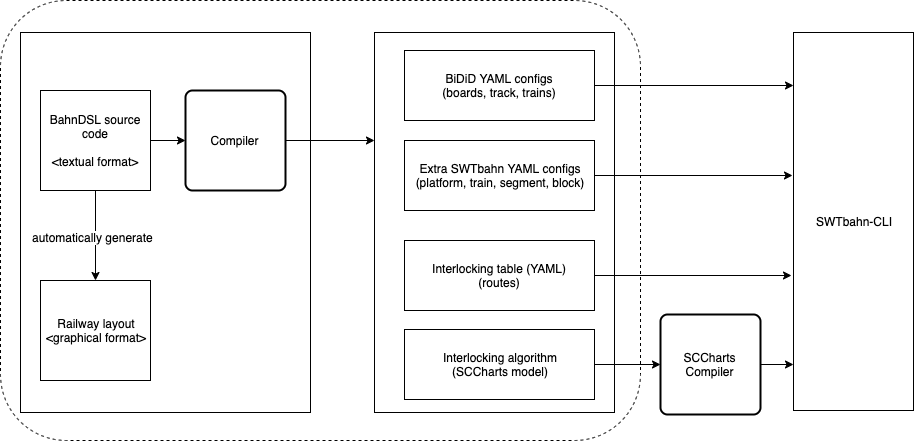
\includegraphics[width=390pt]{diagrams/bahndsl-overview.png}
    \label{fig:overview}
    \caption{Overview of the product and integration with SWTbahn-CLI}
\end{figure}

The figure \ref{fig:overview} shows the major components of the project and the SWTbahn-CLI integration. This project shall implements all the components inside the rounded box in the left, which contains:
\begin{itemize}
    \item BahnDSL language definition (textual format)
    \item Graphical representation of railway layout
    \item Compiler/IDE for the language
    \item Generated BiDiB YAML configuration files: boards, track, trains
    \item Generated Extra SWTbahn YAML configuration files (which contains additional information of BiDiB configuration files) for: platform, train, segment, block
    \item Generated interlocking table (YAML file)
    \item Generated interlocking algorithm (SCCharts model)
\end{itemize}

All generated configuration files and interlocking table shall be used directly in an existing application called SWTbahn-CLI for configuring the railway model. The SCCharts model which represents the interlocking algorithm must be compiled using an external compiler tool (Kieler Compiler) to generate low-level C code before being used in SWTbahn-CLI application.

\section{Product Functions}

\begin{itemize}
    \item IDE
    \begin{itemize}
        \item General Eclipse-based IDE features (project management, code editing, ...)
        \item Generate graphical representation of railway layout during development
    \end{itemize}
    \item Compiler
    \begin{itemize}
        \item Input: Collection of BahnDSL source files
        \item Output:
        \begin{itemize}
            \item BiDiB configuration files
            \item Extra SWTbahn configuration files
            \item Interlocking table
            \item Interlocking algorithm
        \end{itemize}
    \end{itemize}
\end{itemize}

\section{User Classes and Characteristics}
\begin{itemize}
    \item Typical users: use the BahnDSL to configure the railway layout, generate interlocking table and interlocking algorithm
\end{itemize}

\section{Operating Environment}

The project shall deliver two software applications which have the same requirement:
\begin{itemize}
    \item Operating System: macOS, Windows, Linux
    \item Java JRE 8 or later
\end{itemize}

\section{Design and Implementation Constraints}
BahnDSL is developed in \href{https://www.eclipse.org/xtend/}{Xtend} (a high-level programming language for the JVM), it uses \href{https://www.eclipse.org/Xtext/}{Xtext plugin} and is built on top of Eclipse RCP product. The \href{https://www.eclipse.org/sirius/}{Eclipse Sirius} technology is used for generating the graphical representation of railway layout.

\section{User Documentation}
\begin{itemize}
    \item BahnDSL language: Grammar and semantics
    \item BahnDSL compiler and IDE manual
    \item Development of BahnDSL project (including IDE and compiler) using Eclipse Xtext, detailed information about development, testing, and deployment
\end{itemize}

% \chapter{External Interface Requirements}

% \section{User Interfaces}
% $<$Describe the logical characteristics of each interface between the software 
% product and the users. This may include sample screen images, any GUI standards 
% or product family style guides that are to be followed, screen layout 
% constraints, standard buttons and functions (e.g., help) that will appear on 
% every screen, keyboard shortcuts, error message display standards, and so on.  
% Define the software components for which a user interface is needed. Details of 
% the user interface design should be documented in a separate user interface 
% specification.$>$

% \section{Hardware Interfaces}
% $<$Describe the logical and physical characteristics of each interface between 
% the software product and the hardware components of the system. This may include 
% the supported device types, the nature of the data and control interactions 
% between the software and the hardware, and communication protocols to be 
% used.$>$

% \section{Software Interfaces}
% $<$Describe the connections between this product and other specific software 
% components (name and version), including databases, operating systems, tools, 
% libraries, and integrated commercial components. Identify the data items or 
% messages coming into the system and going out and describe the purpose of each.  
% Describe the services needed and the nature of communications. Refer to 
% documents that describe detailed application programming interface protocols.  
% Identify data that will be shared across software components. If the data 
% sharing mechanism must be implemented in a specific way (for example, use of a 
% global data area in a multitasking operating system), specify this as an 
% implementation constraint.$>$

% \section{Communications Interfaces}
% $<$Describe the requirements associated with any communications functions 
% required by this product, including e-mail, web browser, network server 
% communications protocols, electronic forms, and so on. Define any pertinent 
% message formatting. Identify any communication standards that will be used, such 
% as FTP or HTTP. Specify any communication security or encryption issues, data 
% transfer rates, and synchronization mechanisms.$>$


\chapter{System Features}

\section{BahnDSL language definition}

\paragraph{}The language shall be able to describe all components of the railway layout and their properties including the connections to each others. Each component contains a unique id and additional values. The associated hardware address might be attached depend on the component type.

\paragraph{}Components and their properties:
\begin{itemize}
    \item Board: list of features, each feature defined by a address number with value
    \item Segment: extra properties represent length, maximum speed, supported train curve
    \item Signal: aspects (red or green) and initial properties
    \item Point: aspects (normal or reverse) and initial properties
    \item Block: Block of segments one main segment and buffer segments (1 or 2)
    \begin{itemize}
        \item Main segment
        \item Buffer segment(s)
        \item Direction: bidirectional, clockwise, anti-clockwise
        \item Entry Signal
        \item Train types: cargo, passenger,...
    \end{itemize}
\end{itemize}

\section{Graphical railway representation}

\paragraph{}Sirius Eclipse shall be used for modelling the railway layout. Based on the description of BahnDSL textual source code, the graphical representation of the railway layout is being rendered in parallel during development.

\paragraph{}The model shall represent the completed layout including all boards and track components described in the textual source code. The trains are excluded from the layout.

\section{BiDiB configuration files generation}

\paragraph{}BiDiB configuration files shall be generated by the compiler. 3 files with pre-defined structure that contains the hardware addresses of components on the platform and addition information:
\begin{itemize}
    \item bidib_board_config.yml
    \item bidib_track_config.yml
    \item bidib_train_config.yml
\end{itemize}

Sample contains of each files are included in the Appendix \ref{appendix_bidib}.

\section{Extra SWTbahn configuration files generation}

\paragraph{}In addition to the BiDiB configuration files, an extra single or multiple configuration files shall be generated to represent more properties of the railway components which describe more aspects of the units. These extra values shall be useful for the interlocking procedure.

\paragraph{}Listing of additional properties for each component:
\begin{itemize}
    \item Platform
    \begin{itemize}
        \item Block
        \item Direction
        \item Supported train types
        \item Length
    \end{itemize}
    \item Train
    \begin{itemize}
        \item Weight
        \item Speed profile
        \item Direction
        \item Length
    \end{itemize}
    \item Segment
    \begin{itemize}
        \item Length
        \item Maximum speed
    \end{itemize}
    \item Block
    \begin{itemize}
        \item Main segment
        \item Buffer segments
        \item Direction
        \item Entry signal
        \item Supported train types
    \end{itemize}
\end{itemize}

\paragraph{}A sample YAML structure is included in Appendix \ref{appendix_extra_config}.

\paragraph{}There are another set of properties that show the relationship between the components to form the completed railway layout. The detailed structure shall be proposed during development.

\section{Interlocking table generation}
\paragraph{}Based on the completed railway layout described by BahnDSL source code, all possible routes from a signal to all other routes shall be computed. Each route from one signal to another signal must contain below properties:
\begin{itemize}
    \item Source signal
    \item Destination signal
    \item Direction
    \item Path (collection of blocks/segments)
    \item Points (collection of points)
    \item Signals (collection of signals)
    \item Conflicts (collection of other routes in the table)
\end{itemize}

\paragraph{}The interlocking table contains all valid routes generated and filtered by the railway layout specified in the BahnDSL source code. The compiler shall generate a YAML configuration file which represents the described interlocking table. A sample YAML structure is included in Appendix \ref{appendix_interlocking_table}.

\section{Interlocking algorithm generation}

\chapter{Other Nonfunctional Requirements}

\section{Performance Requirements}
BahnDSL project does not have any performance requirements.

\section{Safety Requirements}
BahnDSL project does not have any safety requirements.

\section{Security Requirements}
BahnDSL project does not have any security requirements.

\section{Software Quality Attributes}
The BahnDSL project provides both IDE application (GUI-based) and command-line application which suit different scenarios. Moreover, the IDE application shall be easy to use for users who are familiar with Eclipse platforms.

\appendix
\chapter{Appendices}

\section{Sample BiDiB configuration files}
\label{appendix_bidib}
\textbf{bidib_board_config.yml}
\begin{lstlisting}[basicstyle=\small]
    boards:
        - id: master
        unique-id: 0xDA000D680052EF
        features:
            # seckack on, 200ms
            - number: 0x03
            value: 0x14
            # track output default off
            - number: 0x6E
            value: 0x00
        - id: lightcontrol
        unique-id: 0x05000D6B0083EC
        - id: onecontrol
        unique-id: 0x05000D7500DBED
\end{lstlisting}

\textbf{bidib_track_config.yml}
\begin{lstlisting}[basicstyle=\small]
    boards:
        - id: master
            segments:
            - id: seg1
                address: 0x00
            - id: seg2
                address: 0x01
        - id: lightcontrol
            signals-board:
                - id: signal1
                number: 0x00
                aspects:
                    - id: yellow
                    value: 0x02
                    - id: green
                    value: 0x01
                    - id: red
                    value: 0x00
                initial: red
        - id: onecontrol
            points-board:
            - id: point1
                number: 0x00
                aspects:
                - id: normal
                    value: 0x01
                - id: reverse
                    value: 0x00
                initial: normal
\end{lstlisting}

\textbf{bidib_train_config.yml}
\begin{lstlisting}[basicstyle=\small]
    trains:
        - id: cargo_db
        dcc-address: 0x0001 # addr high | addr low
        dcc-speed-steps: 126
        calibration:
            - 5
            - 15
            - 30
            - 45
            - 60
            - 75
            - 90
            - 105
            - 120
        peripherals:
            - id: head_light
            bit: 4          # a value in range 0..31
            initial: 1
            - id: light_carriage
            bit: 0          # a value in range 0..31
            initial: 1
\end{lstlisting}

\section{Sample extra SWTbahn configuration files}
\label{appendix_extra_config}
\begin{lstlisting}[basicstyle=\small]
# Extra platform configuration
platforms:
  - id: platform1
    block_id: block1
    exit_direction: clockwise
    train_types:
      - cargo
      - passenger
    length: 35 # cm

# Extra train configuration (in addition to bidid_train_config)
trains:
  - id: cargo_db
    weight: 30 # tons
    length: 20 # cm
    speed_profile: to be determined

# Extra track configuration (in addition to bidid_track_config)
segments:
  - id: seg1
  - length: 25cm # cm
  - max_speed: 100
  - train_curve: to be determined

# Define blocks
blocks:
  - id: block1
    main_segment: seg1
    buffer_segments:
      - seg2
      - seg3
    direction: bidirectional # clockwise, anti-clockwise
    entry_signal: signal1
    train_types:
      - cargo
      - passenger
\end{lstlisting}

\section{Appendix C: Sample interlocking table}
\label{appendix_interlocking_table}
\begin{lstlisting}[basicstyle=\small]
interlocking-table:
    - id: 0
      source: signal3a
      destination: signal6
      direction: anti-clockwise
      path:
        - id: seg31
        - id: seg30
          end: seg29
      points:
        - id: point2
          position: reverse
      signals:
        - id: signal5
      conflicts:
        - id: 1
        - id: 2
        - id: 3
        - id: 4
        - id: 5
        - id: 6
        - id: 7
        - id: 8
        - id: 9
\end{lstlisting}
\end{document}
